\chapter{Compressione lossless di immagini}

La compressione lossless di immagini è richiesta in applicazioni dove le immagini sono soggette ad ulteriori operazioni, editing o compressioni/decompressioni ripetute. Inoltre viene effettuata anche dove ottenere le immagini è molto costoso, come nel caso di immagini extraterrestri o immagini mediche. Generalmente la compressione lossless è possibile in quanto spesso le immagini contengono ridondanze che possono essere sfruttate per ridurre le dimensioni dell'immagine stessa.

Lo schema di compressione può essere diviso in due fasi:

\begin{itemize}
    \item \textbf{Modeling}: nel quale la ridondanza dei dati viene analizzata e rappresentata come un modello (ovvero si cambia la rappresentazione dei dati);
    \item \textbf{Coding}: nel quale viene codificata la differenza tra i veri e propri dati e il modello.
\end{itemize}

\begin{figure}[htbp!]
  \centering
  \includesvg[inkscapelatex=false, width = 430pt]{5.1}
\end{figure}
\FloatBarrier

Spesso queste due fasi possono essere eseguite in parallelo. Un'immagine è osservata campione per campione in un ordine predefinito (normalmente in raster scan), e l'obiettivo della fase di modeling è quello di ottenere informazioni sui dati nella forma di modello probabilistico, che viene usato successivamente per la fase di coding.

Questa fase può essere vista come un problema di inferenza induttiva, nel quale in ogni istante \(t\), e dopo aver esaminato i dati \(x^t = x_1 x_2 \dots x_t\), si prova a capire che inferenza abbiano sul prossimo campione \(x_{t+1}\) assegnando una distribuzione di probabilità condizionata \(P(\cdot |x^t)\). Idealmente la lunghezza del codice del campione \(x_{t+1}\) è \(- \log P(x_{t+1}|x^t)\), che è molto vicina alla media dell'entropia del modello probabilistico.

\section{Strategia di modeling}

La maggior parte degli schemi sono basati su una strategia di modeling nella quale gli assegnamenti adattivi di probabilità sono divisi in diverse componenti:
\begin{enumerate}
    \item Un passo di predizione, nel quale viene predetto un valore \(\hat{x}_{t+1}\) per il prossimo campione \(x_{t+1}\) e questo valore è basato su un sottoinsieme finito (detto \textit{causal template}) dei dati passati disponibili.
    \item Viene poi determinato un contesto nel quale è presente \(x_{t+1}\). Il contesto è una funzione del possibile casual template.
    \item Viene stabilito un modello probabilistico per il residuo di predizione (\textit{error signal}): \(\epsilon_{t+1} = x_{t+1} - \hat{x}_{t+1}\), che ha condizionato il contesto di \(x_{t+1}\).
\end{enumerate}

Il residuo di predizione è basato sulla distribuzione di probabilità stabilita nello step 3. Sia la predizione, che il contesto, che la distribuzione di probabilità sono egualmente disponibili anche al decompressore, che può quindi recuperare il valore esatto che è stato compresso. Questo processo è particolarmente utile in situazioni dove i campioni rappresentano una misura fisica che cambia continuamente, e il valore del prossimo campione può essere quindi predetto accuratamente utilizzando una semplice funzione lineare dei suoi campioni vicini. 

Livelli più bassi di entropia possono essere ottenuti attraverso contesti più grandi, catturando le dipendenze high-order, ma il risparmio di entropia potrebbe essere compensato da un costo del modello. Questo costo cattura le penalità di    \textit{context dilution} che si verificano quando le statistiche di conteggio devono essere distribuite su troppi contesti, influenzando così la precisione delle stime corrispondenti. Per bilanciare la suddetta "tensione" tra risparmio di entropia e costo del modello, la scelta del modello dovrebbe essere guidata dall'uso, quando possibile, della conoscenza precedente disponibile sui dati da modellare, evitando inutili costi di apprendimento, come l'overfitting.


Questo spiega il relativo fallimento di tool universali di compressione basati solo su algoritmi standard di sostituzione o statistici, in quanto quando vengono applicati a scenari reali non sempre si comportano come dovrebbero.


\section{Lossless JPEG}
Lo standard JPEG fu introdotto verso la fine degli anni '80 per facilitare la diffusione delle macchine fotografiche digitali, quando ISO, CCITT e IEC crearono il Joint Photographic Experts Group per sviluppare appunto uno standard per la compressione e la decompressione di immagini.

Lo standard JPEG include quattro metodi di compressione: tre di questi lossy (sequential encoding, progressive encoding, hierarchical encoding), che sono basati sulla trasformata discreta del coseno (DCT) e una lossless che non fu oggetto di studi approfonditi e fu abbandonata, basato parzialmente su un algoritmo di compressione chiamato Sunset. 

\vspace{5mm}

Lossless JPEG si basa sulla strategia che abbiamo appena visto, ovvero sulla predizione del prossimo campione. Tranne alcuni casi particolari, questo casual template prevede i tre pixel al di sopra, a sinistra e diagonalmente rispetto a \(x\). In generale la scelta di \(x\) dipende dalla scelta del predittore, e normalmente lossless JPEG utilizza il numero 7 come default.

\begin{table}[htbp!]
\centering
\begin{tabular}{|c|c|c|c|c|cc} 
\cline{6-7}
\multicolumn{1}{l}{} & \multicolumn{1}{l}{} & \multicolumn{1}{l}{} & \multicolumn{1}{l}{} & \multicolumn{1}{l}{} & \textbf{Selection value} & \textbf{Prediction}  \\ 
\cline{6-7}
\multicolumn{1}{c}{} & \multicolumn{1}{c}{} & \multicolumn{1}{c}{} & \multicolumn{1}{c}{} & \multicolumn{1}{c}{} & 0                        & no prediction        \\
\multicolumn{1}{c}{} & \multicolumn{1}{c}{} & \multicolumn{1}{c}{} & \multicolumn{1}{c}{} & \multicolumn{1}{c}{} & 1                        & A                    \\
\multicolumn{1}{c}{} & \multicolumn{1}{c}{} & \multicolumn{1}{c}{} & \multicolumn{1}{c}{} & \multicolumn{1}{c}{} & 2                        & B                    \\
\multicolumn{1}{c}{} & \multicolumn{1}{c}{} & \multicolumn{1}{c}{} & \multicolumn{1}{c}{} & \multicolumn{1}{c}{} & 3                        & C                    \\ 
\cline{1-5}
                     &                      &                      &                      &                      & 4                        & A + B - C            \\ 
\cline{1-5}
                     & C                    & B                    &                      &                      & 5                        & A + ((B - C) / 2)    \\ 
\cline{1-5}
                     & A                    & X                    &                      &                      & 6                        & B + ((A - C) / 2)    \\ 
\cline{1-5}
                     &                      &                      &                      &                      & 7                        & (A + B) / 2          \\
\cline{1-5}
\end{tabular}
\end{table}
\FloatBarrier

Per comprimere un pixel X con lossless JPEG si utilizza uno dei predittori e si sottrae il valore ottenuto al valore di X. Il risultato solitamente è un numero piccolo, che poi viene codificato entropicamente via Huffman o Arithmetic Coding.

Lossless JPEG produce fattori di compressione di 2 a 1 o meno, quindi è inferiore ad altri metodi di compressione lossless di immagini.

\section{FELICS}
L'algoritmo FELICS (Fast, Efficient Lossless Image Compression System) può essere considerato un primo passo per colmare il divario di compressione tra gli schemi guidati dalla semplicità e gli schemi basati sulla modellazione del contesto e la codifica aritmetica, poiché incorpora l'adattabilità in una struttura a bassa complessità.
La sua compressione su immagini fotografiche non è lontana da quella fornita da lossless JPEG (versione con Arithmetic coding), e il codice è riportato per funzionare fino a cinque volte più veloce. Per ragioni di complessità FELICS evita l'utilizzo di arithmetic code e usa almeno un bit per codificare per ogni campione. Per cui non funziona bene sulle immagini che possono essere compresse molto.  

\begin{figure}[htbp!]
  \centering
  \includesvg[inkscapelatex=true, width = \textwidth]{5.2}
\end{figure}
\FloatBarrier
%INSERIRE IMMAGINE FELICS 5.2 svg

Consideriamo i vicini A e B di un pixel P. Usiamo A,B e P per indicare sia i tre pixel sia le loro intensità di grigio. Indichiamo con L e H i vicini con intensità minore e maggiore rispettivamente. Distinguiamo tre casi:

\begin{enumerate}
    \item L'intensità del pixel P è tra L ed H (ovvero nella regione centrale della figura). Questo caso si verifica più o meno nella metà dei pixel, e in questo caso a P è assegnata una codifica che inizia con 0.
    \item L'intensità di P è minore di L, e la codifica assegnata inizia con 10.
    \item L'intensità di P è maggiore di H, e la codifica assegnata inizia con 11.
\end{enumerate}

Quando P è in una delle regioni esterne, la probabilità che la sua intensità sia molto diversa da L e da H è molto bassa, per cui a P può essere assegnata una codifica più lunga. La codifica di P dipende quindi in maniera elevata dalla posizione di P nel grafico. 

Abbiamo bisogno di \(H - L + 1\) codici a lunghezza variabile. Poniamo \(k = \lfloor \log_2 (H - L + 1) \rfloor\) e calcoliamo gli interi \(a\) e \(b\) in questo modo:

\[a = 2^{k+1} - (H - L + 1),  b = 2(H - L + 1 - 2^k)\]

\vspace{5mm}

\textbf{Esempio:} sia \(L = 5\) e \(H = 24\). Le codifiche per alcuni pixel \(P\) sono mostrate nella tabella:

\begin{table}[htbp!]
\centering
\begin{tabular}{rcl}
\multicolumn{1}{c}{\textbf{Pixel P}} & \textbf{Region code} & \multicolumn{1}{c}{\textbf{Pixel code}}  \\ 
\hline
L = 15                               & 0                    & 0000                                     \\
16                                   & 0                    & 0010                                     \\
17                                   & 0                    & 010                                      \\
18                                   & 0                    & 011                                      \\
19                                   & 0                    & 100                                      \\
20                                   & 0                    & 101                                      \\
21                                   & 0                    & 110                                      \\
22                                   & 0                    & 111                                      \\
23                                   & 0                    & 0001                                     \\
H = 24                               & 0                    & 0011                                    
\end{tabular}
\end{table}
\FloatBarrier

\section{JPEG-LS}
La standardizzazione di JPEG-LS inizia nel 1994 e viene portata avanti attraverso i contributi di diversi produttori di apparecchiature elettroniche per la produzione di immagini insieme a università e industrie. Furono presentate nove proposte, delle cui vinse LOCO-I, algoritmo presentato da HP, chiamato successivamente JPEG-LS. Oggi viene utilizzato in tutti i campi, compreso quello medico. Lo scopo è quello di ottenere il bilanciamento migliore tra compressione ottima e complessità computazionale bassa. In realtà una delle proposte, CALIC, che aveva una complessità maggiore di LOCO-I, otteneva una compressione migliore, ma fu scelto appunto LOCO-I per il miglior bilanciamento tra le due caratteristiche.

\vspace{5mm}

L'algoritmo JPEG-LS esamina alcuni vicini del pixel corrente e li utilizza come contesto che verrà utilizzato per predire il valore di quel pixel e per selezionare una distribuzione di probabilità che verrà usata per codificare la differenza di predizione rispetto al valore del pixel, utilizzando Golomb. Inoltre è presente una modalità di funzionamento chiamata \textit{run mode}, che viene utilizzata quando sono presenti più pixel che hanno lo stesso valore e permette di codificare la lunghezza di questa "lista" di pixel uguali piuttosto che codificarli uno ad uno.

Il contesto definito per codificare un pixel \(X\) è l'insieme dei pixel a sinistra di \(X\) (\(W\)), in alto a sinistra \(NW\), sopra \(N\) e in alto a destra \(NE\). Il codificatore esamina i pixel del contesto e decide se codificare il pixel \(X\) in \textit{run mode} oppure in \textit{regular mode}.

\vspace{4mm}

\begin{figure}[htbp!]
\centering
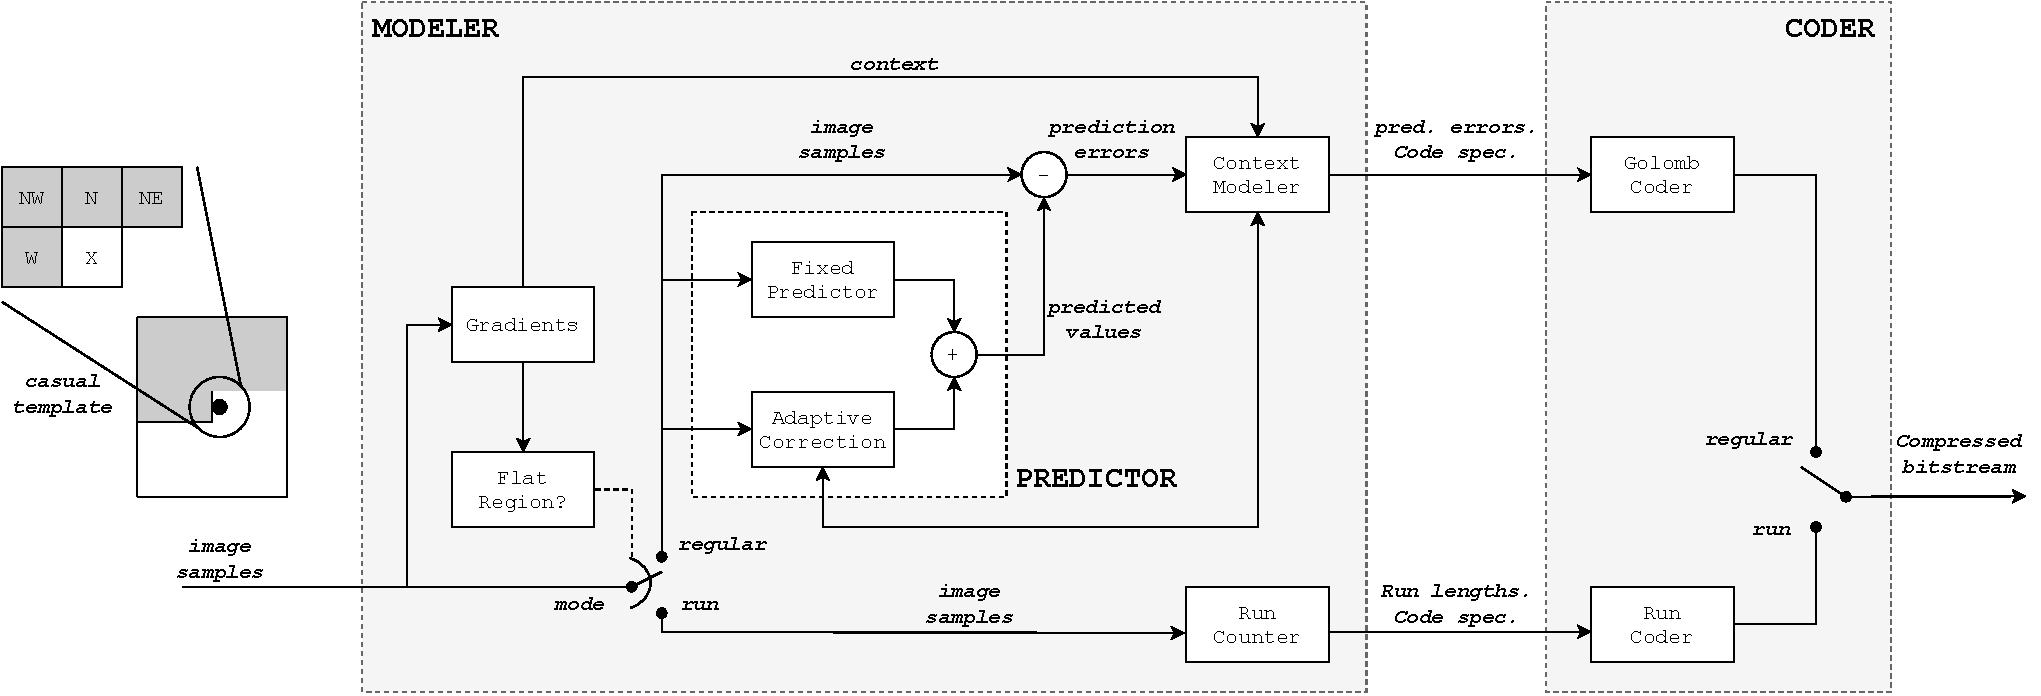
\includegraphics[width=\textwidth]{Images/5.3.pdf}
\end{figure}
\FloatBarrier

\vspace{4mm}

%\begin{figure}[htbp!]
%  \centering
%  \includesvg[inkscapelatex=false, width = \textwidth]{5.3}
%\end{figure}
%\FloatBarrier

\textbf{Run mode} \(\>\>\) Si conta la lunghezza della sequenza e tramite il \textbf{run coder} si codifica questo valore. Infine si invia al decompressore, che sa di trovarsi in run mode e decodifica il valore, inviandolo in output.

\textbf{Regular mode} \(\>\>\) Viene calcolata una predizione del valore di \(X\) tramite il \textbf{fixed predictor}, che utilizza una funzione chiamata \textit{Median Edge Detector} (MED):

\[\hat{x}_{MED} = min(I_w, I_n, I_{nw}) + max(I_w, I_n, I_{nw}) - I_{nw}\]

Una volta calcolato questo valore, tramite l'\textbf{adaptive correction} si ottiene una correzione con un termine che dipende dal contesto, che viene codificato tramite la codifica di Golomb. 

Per codificare si utilizza un modello di probabilità che evita il problema della \textit{context dilution}, ovvero cerca di creare meno contesti possibili, attraverso l'utilizzo di \textbf{gradients}, che stimano il valore da dare al codice di Golomb. Il codice di Golomb poi dipende da tutti e quattro i pixel del contesto e dall'errore di predizione che era stato codificato precedentemente per lo stesso contesto.


\let\cleardoublepage\clearpage